\documentclass[twoside]{book}

% Packages required by doxygen
\usepackage{calc}
\usepackage{doxygen}
\usepackage{graphicx}
\usepackage[utf8]{inputenc}
\usepackage{makeidx}
\usepackage{multicol}
\usepackage{multirow}
\usepackage{textcomp}
\usepackage[table]{xcolor}

% NLS support packages
\usepackage[french]{babel}

% Font selection
\usepackage[T1]{fontenc}
\usepackage{mathptmx}
\usepackage[scaled=.90]{helvet}
\usepackage{courier}
\usepackage{amssymb}
\usepackage{sectsty}
\renewcommand{\familydefault}{\sfdefault}
\allsectionsfont{%
  \fontseries{bc}\selectfont%
  \color{darkgray}%
}
\renewcommand{\DoxyLabelFont}{%
  \fontseries{bc}\selectfont%
  \color{darkgray}%
}

% Page & text layout
\usepackage{geometry}
\geometry{%
  a4paper,%
  top=2.5cm,%
  bottom=2.5cm,%
  left=2.5cm,%
  right=2.5cm%
}
\tolerance=750
\hfuzz=15pt
\hbadness=750
\setlength{\emergencystretch}{15pt}
\setlength{\parindent}{0cm}
\setlength{\parskip}{0.2cm}
\makeatletter
\renewcommand{\paragraph}{%
  \@startsection{paragraph}{4}{0ex}{-1.0ex}{1.0ex}{%
    \normalfont\normalsize\bfseries\SS@parafont%
  }%
}
\renewcommand{\subparagraph}{%
  \@startsection{subparagraph}{5}{0ex}{-1.0ex}{1.0ex}{%
    \normalfont\normalsize\bfseries\SS@subparafont%
  }%
}
\makeatother

% Headers & footers
\usepackage{fancyhdr}
\pagestyle{fancyplain}
\fancyhead[LE]{\fancyplain{}{\bfseries\thepage}}
\fancyhead[CE]{\fancyplain{}{}}
\fancyhead[RE]{\fancyplain{}{\bfseries\leftmark}}
\fancyhead[LO]{\fancyplain{}{\bfseries\rightmark}}
\fancyhead[CO]{\fancyplain{}{}}
\fancyhead[RO]{\fancyplain{}{\bfseries\thepage}}
\fancyfoot[LE]{\fancyplain{}{}}
\fancyfoot[CE]{\fancyplain{}{}}
\fancyfoot[RE]{\fancyplain{}{\bfseries\scriptsize Généré le Jeudi 23 Avril 2015 11\-:19\-:28 pour project\-\_\-trading\-\_\-doc par Doxygen }}
\fancyfoot[LO]{\fancyplain{}{\bfseries\scriptsize Généré le Jeudi 23 Avril 2015 11\-:19\-:28 pour project\-\_\-trading\-\_\-doc par Doxygen }}
\fancyfoot[CO]{\fancyplain{}{}}
\fancyfoot[RO]{\fancyplain{}{}}
\renewcommand{\footrulewidth}{0.4pt}
\renewcommand{\chaptermark}[1]{%
  \markboth{#1}{}%
}
\renewcommand{\sectionmark}[1]{%
  \markright{\thesection\ #1}%
}

% Indices & bibliography
\usepackage{natbib}
\usepackage[titles]{tocloft}
\setcounter{tocdepth}{3}
\setcounter{secnumdepth}{5}
\makeindex

% Hyperlinks (required, but should be loaded last)
\usepackage{ifpdf}
\ifpdf
  \usepackage[pdftex,pagebackref=true]{hyperref}
\else
  \usepackage[ps2pdf,pagebackref=true]{hyperref}
\fi
\hypersetup{%
  colorlinks=true,%
  linkcolor=blue,%
  citecolor=blue,%
  unicode%
}

% Custom commands
\newcommand{\clearemptydoublepage}{%
  \newpage{\pagestyle{empty}\cleardoublepage}%
}


%===== C O N T E N T S =====

\begin{document}

% Titlepage & ToC
\hypersetup{pageanchor=false}
\pagenumbering{roman}
\begin{titlepage}
\vspace*{7cm}
\begin{center}%
{\Large project\-\_\-trading\-\_\-doc }\\
\vspace*{1cm}
{\large Généré par Doxygen 1.8.6}\\
\vspace*{0.5cm}
{\small Jeudi 23 Avril 2015 11:19:28}\\
\end{center}
\end{titlepage}
\clearemptydoublepage
\tableofcontents
\clearemptydoublepage
\pagenumbering{arabic}
\hypersetup{pageanchor=true}

%--- Begin generated contents ---
\chapter{Index hiérarchique}
\section{Hiérarchie des classes}
Cette liste d'héritage est classée approximativement par ordre alphabétique \-:\begin{DoxyCompactList}
\item Q\-Dialog\begin{DoxyCompactList}
\item \contentsline{section}{Aide}{\pageref{class_aide}}{}
\item \contentsline{section}{Config}{\pageref{class_config}}{}
\item \contentsline{section}{Faq}{\pageref{class_faq}}{}
\item \contentsline{section}{Help}{\pageref{class_help}}{}
\end{DoxyCompactList}
\item Q\-Main\-Window\begin{DoxyCompactList}
\item \contentsline{section}{Main\-Window}{\pageref{class_main_window}}{}
\end{DoxyCompactList}
\item Q\-Object\begin{DoxyCompactList}
\item \contentsline{section}{Connection\-D\-B}{\pageref{class_connection_d_b}}{}
\end{DoxyCompactList}
\end{DoxyCompactList}

\chapter{Index des classes}
\section{Liste des classes}
Liste des classes, structures, unions et interfaces avec une brève description \-:\begin{DoxyCompactList}
\item\contentsline{section}{{\bf Aide} }{\pageref{class_aide}}{}
\item\contentsline{section}{{\bf Config} }{\pageref{class_config}}{}
\item\contentsline{section}{{\bf Connection\-D\-B} }{\pageref{class_connection_d_b}}{}
\item\contentsline{section}{{\bf Faq} }{\pageref{class_faq}}{}
\item\contentsline{section}{{\bf Help} }{\pageref{class_help}}{}
\item\contentsline{section}{{\bf Main\-Window} }{\pageref{class_main_window}}{}
\end{DoxyCompactList}

\chapter{Index des fichiers}
\section{Liste des fichiers}
Liste de tous les fichiers avec une brève description \-:\begin{DoxyCompactList}
\item\contentsline{section}{\hyperlink{aide_8cpp}{aide.\-cpp} }{\pageref{aide_8cpp}}{}
\item\contentsline{section}{\hyperlink{aide_8h}{aide.\-h} }{\pageref{aide_8h}}{}
\item\contentsline{section}{\hyperlink{config_8cpp}{config.\-cpp} }{\pageref{config_8cpp}}{}
\item\contentsline{section}{\hyperlink{config_8h}{config.\-h} }{\pageref{config_8h}}{}
\item\contentsline{section}{\hyperlink{connectiondb_8cpp}{connectiondb.\-cpp} }{\pageref{connectiondb_8cpp}}{}
\item\contentsline{section}{\hyperlink{connectiondb_8h}{connectiondb.\-h} }{\pageref{connectiondb_8h}}{}
\item\contentsline{section}{\hyperlink{faq_8cpp}{faq.\-cpp} }{\pageref{faq_8cpp}}{}
\item\contentsline{section}{\hyperlink{faq_8h}{faq.\-h} }{\pageref{faq_8h}}{}
\item\contentsline{section}{\hyperlink{help_8cpp}{help.\-cpp} }{\pageref{help_8cpp}}{}
\item\contentsline{section}{\hyperlink{help_8h}{help.\-h} }{\pageref{help_8h}}{}
\item\contentsline{section}{\hyperlink{main_8cpp}{main.\-cpp} }{\pageref{main_8cpp}}{}
\item\contentsline{section}{\hyperlink{mainwindow_8cpp}{mainwindow.\-cpp} }{\pageref{mainwindow_8cpp}}{}
\item\contentsline{section}{\hyperlink{mainwindow_8h}{mainwindow.\-h} }{\pageref{mainwindow_8h}}{}
\end{DoxyCompactList}

\chapter{Documentation des classes}
\section{Référence de la classe Aide}
\label{class_aide}\index{Aide@{Aide}}
Graphe d'héritage de Aide\-:\begin{figure}[H]
\begin{center}
\leavevmode
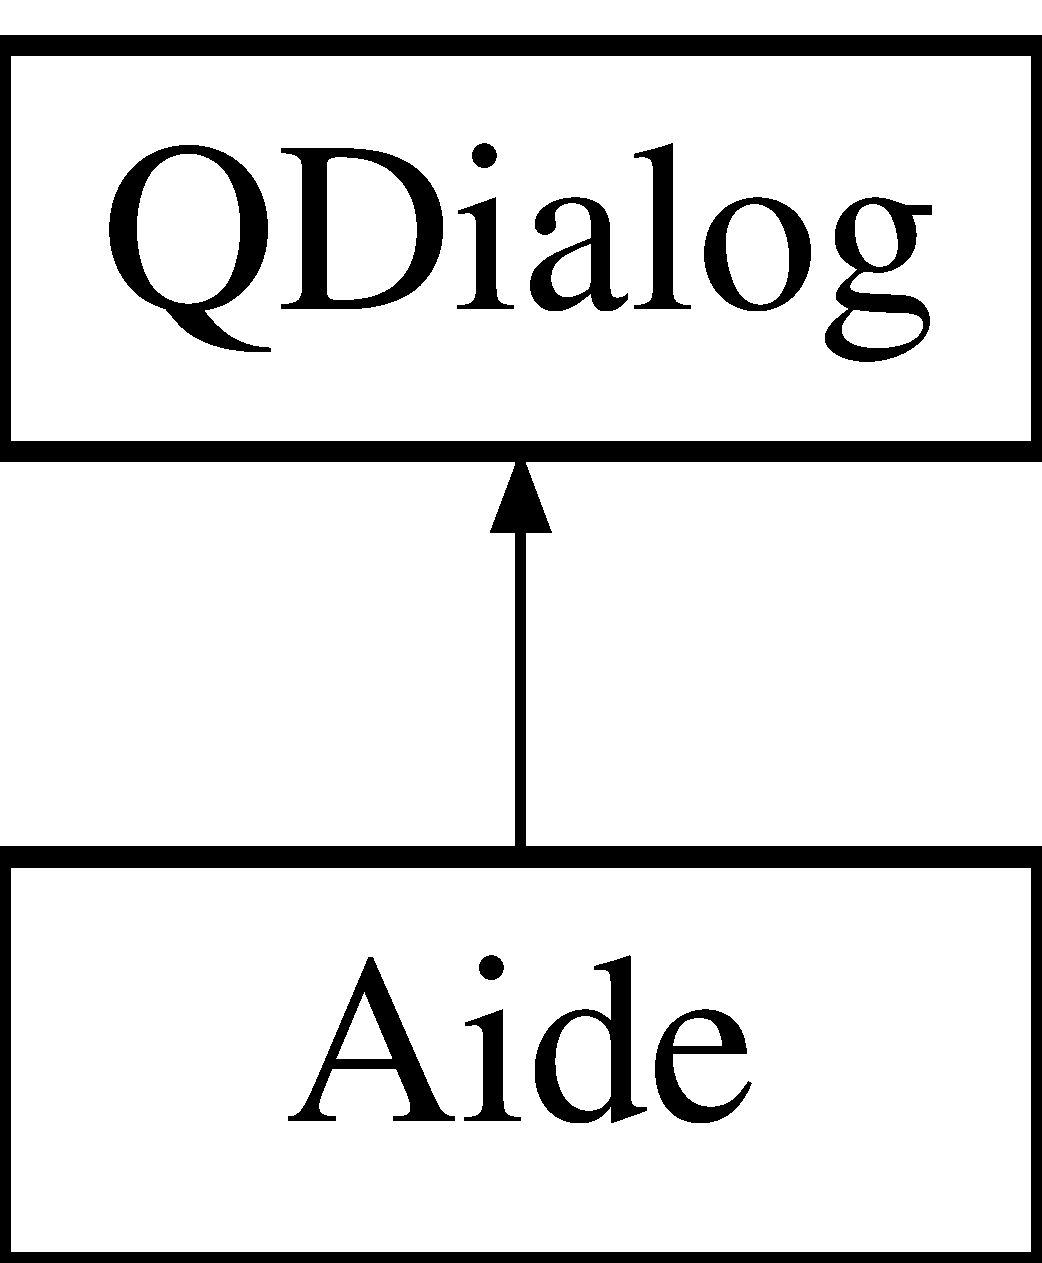
\includegraphics[height=2.000000cm]{class_aide}
\end{center}
\end{figure}


La documentation de cette classe a été générée à partir des fichiers suivants \-:\begin{DoxyCompactItemize}
\item 
aide.\-h\item 
aide.\-cpp\end{DoxyCompactItemize}

\section{Référence de la classe Config}
\label{class_config}\index{Config@{Config}}
Graphe d'héritage de Config\-:\begin{figure}[H]
\begin{center}
\leavevmode
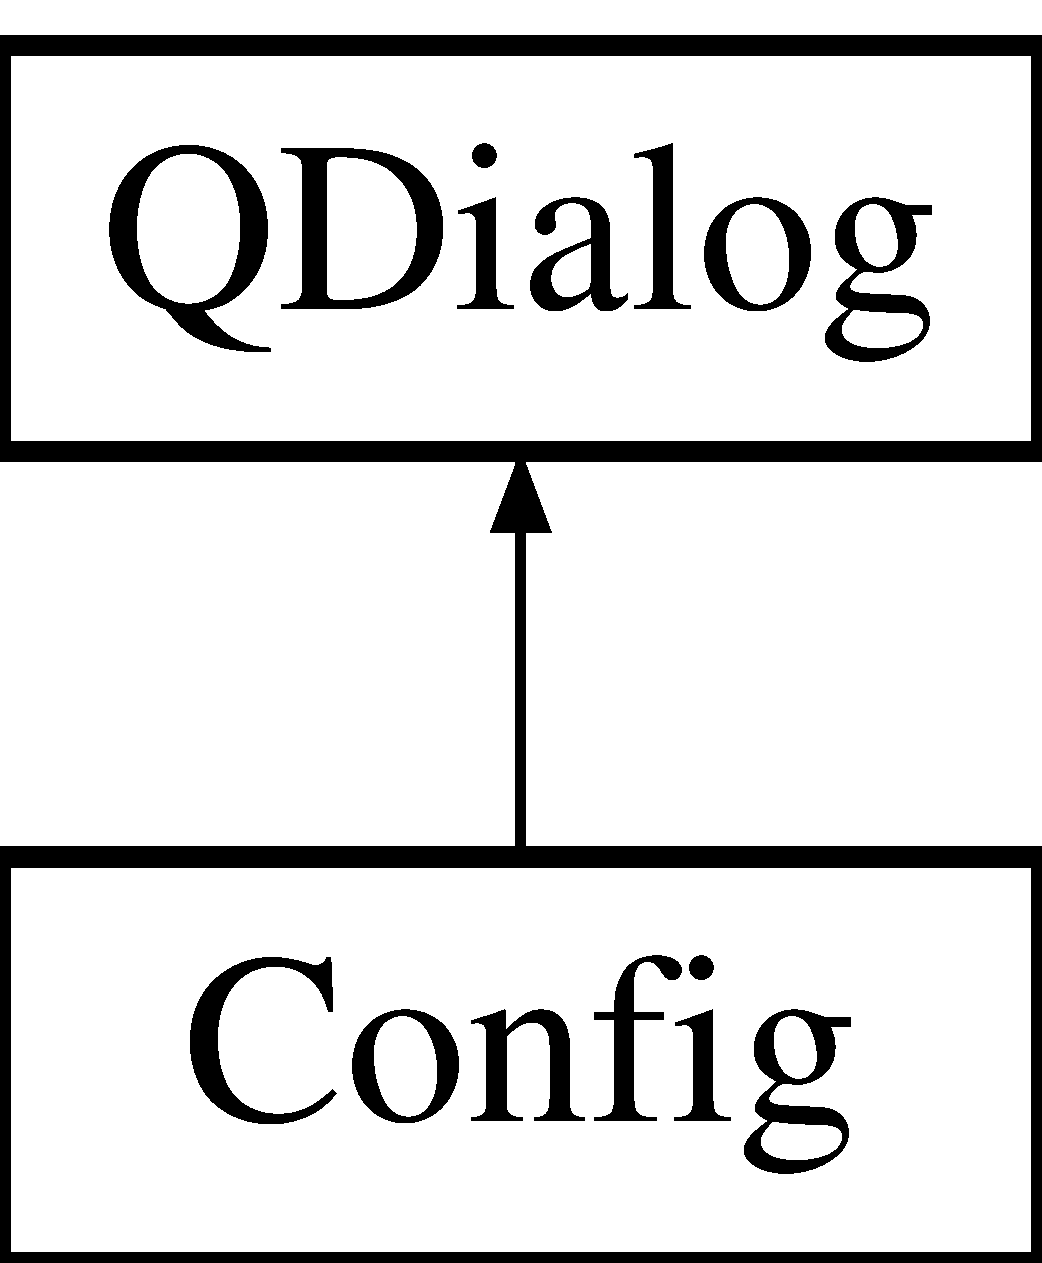
\includegraphics[height=2.000000cm]{class_config}
\end{center}
\end{figure}
\subsection*{Fonctions membres publiques}
\begin{DoxyCompactItemize}
\item 
{\bf Config} (Q\-Widget $\ast$parent)
\end{DoxyCompactItemize}


\subsection{Documentation des constructeurs et destructeur}
\index{Config@{Config}!Config@{Config}}
\index{Config@{Config}!Config@{Config}}
\subsubsection[{Config}]{\setlength{\rightskip}{0pt plus 5cm}Config\-::\-Config (
\begin{DoxyParamCaption}
\item[{Q\-Widget $\ast$}]{parent = {\ttfamily 0}}
\end{DoxyParamCaption}
)}\label{class_config_aae0ecaab37f2ef5794bd0ccbf992e6fc}
Titre de la fenetre

Bouton pour fermer la fenetre d'aide

Slot de fermeture avec le bouton

Affichage du texte et du bouton 

La documentation de cette classe a été générée à partir des fichiers suivants \-:\begin{DoxyCompactItemize}
\item 
config.\-h\item 
config.\-cpp\end{DoxyCompactItemize}

\section{Référence de la classe Connection\-D\-B}
\label{class_connection_d_b}\index{Connection\-D\-B@{Connection\-D\-B}}
Graphe d'héritage de Connection\-D\-B\-:\begin{figure}[H]
\begin{center}
\leavevmode
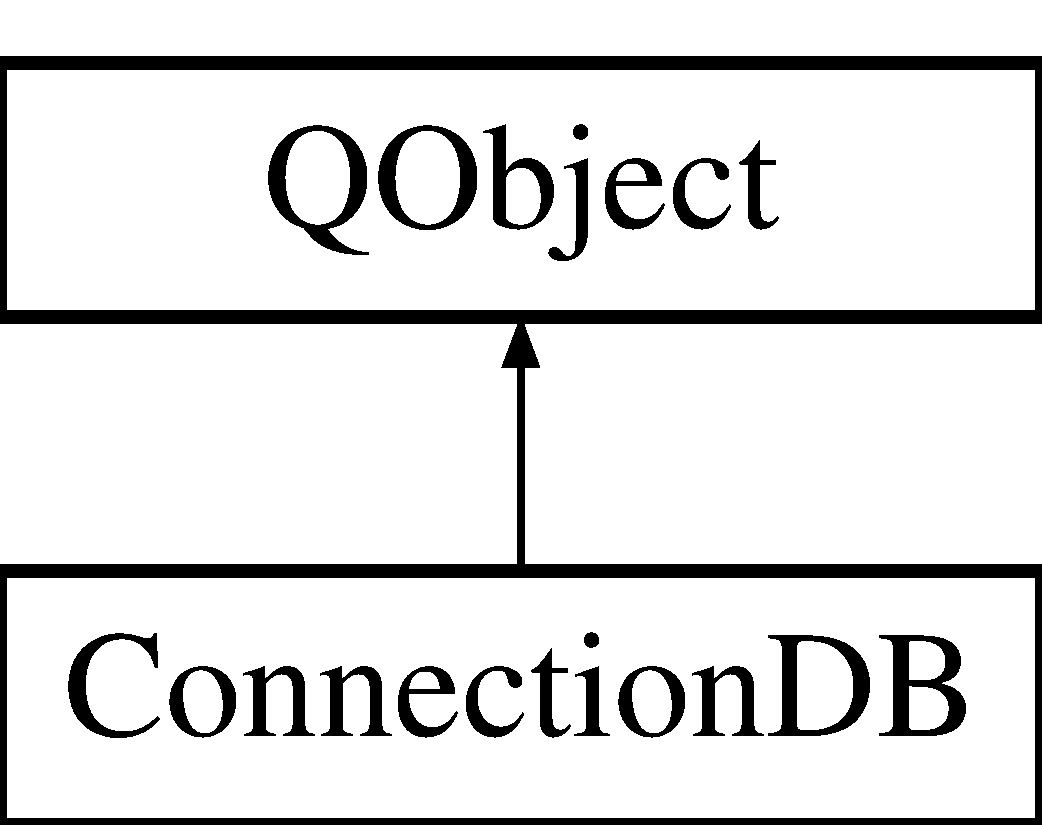
\includegraphics[height=2.000000cm]{class_connection_d_b}
\end{center}
\end{figure}
\subsection*{Fonctions membres publiques}
\begin{DoxyCompactItemize}
\item 
{\bf Connection\-D\-B} (Q\-Widget $\ast$parent, Q\-String debut, Q\-String fin, Q\-String devise)
\begin{DoxyCompactList}\small\item\em Cette classe permet d'etablir une connection a la base de donnee Créer une table si elle n'existe pas. \subsubsection*{Permet d'afficher la table avec les champs demander via une requete }



 \end{DoxyCompactList}\end{DoxyCompactItemize}


\subsection{Documentation des constructeurs et destructeur}
\index{Connection\-D\-B@{Connection\-D\-B}!Connection\-D\-B@{Connection\-D\-B}}
\index{Connection\-D\-B@{Connection\-D\-B}!ConnectionDB@{Connection\-D\-B}}
\subsubsection[{Connection\-D\-B}]{\setlength{\rightskip}{0pt plus 5cm}Connection\-D\-B\-::\-Connection\-D\-B (
\begin{DoxyParamCaption}
\item[{Q\-Widget $\ast$}]{parent, }
\item[{Q\-String}]{debut, }
\item[{Q\-String}]{fin, }
\item[{Q\-String}]{devise}
\end{DoxyParamCaption}
)}\label{class_connection_d_b_aa284d0a538ae540a5b4df55ef88cc13e}


Cette classe permet d'etablir une connection a la base de donnee Créer une table si elle n'existe pas. \subsubsection*{Permet d'afficher la table avec les champs demander via une requete }



 

\subsubsection*{Ize\-Nogoud }

\begin{DoxyDate}{Date}
24 Mars 2015 
\end{DoxyDate}
Connection database

Crée la table \char`\"{}devise\-Table\char`\"{} si elle n'existe pas

Requete S\-Q\-L

Initialise le tableau a afficher

Affiche le tableau avec les données récupérées de la base de données 

La documentation de cette classe a été générée à partir des fichiers suivants \-:\begin{DoxyCompactItemize}
\item 
connectiondb.\-h\item 
connectiondb.\-cpp\end{DoxyCompactItemize}

\section{Référence de la classe Faq}
\label{class_faq}\index{Faq@{Faq}}
Graphe d'héritage de Faq\-:\begin{figure}[H]
\begin{center}
\leavevmode
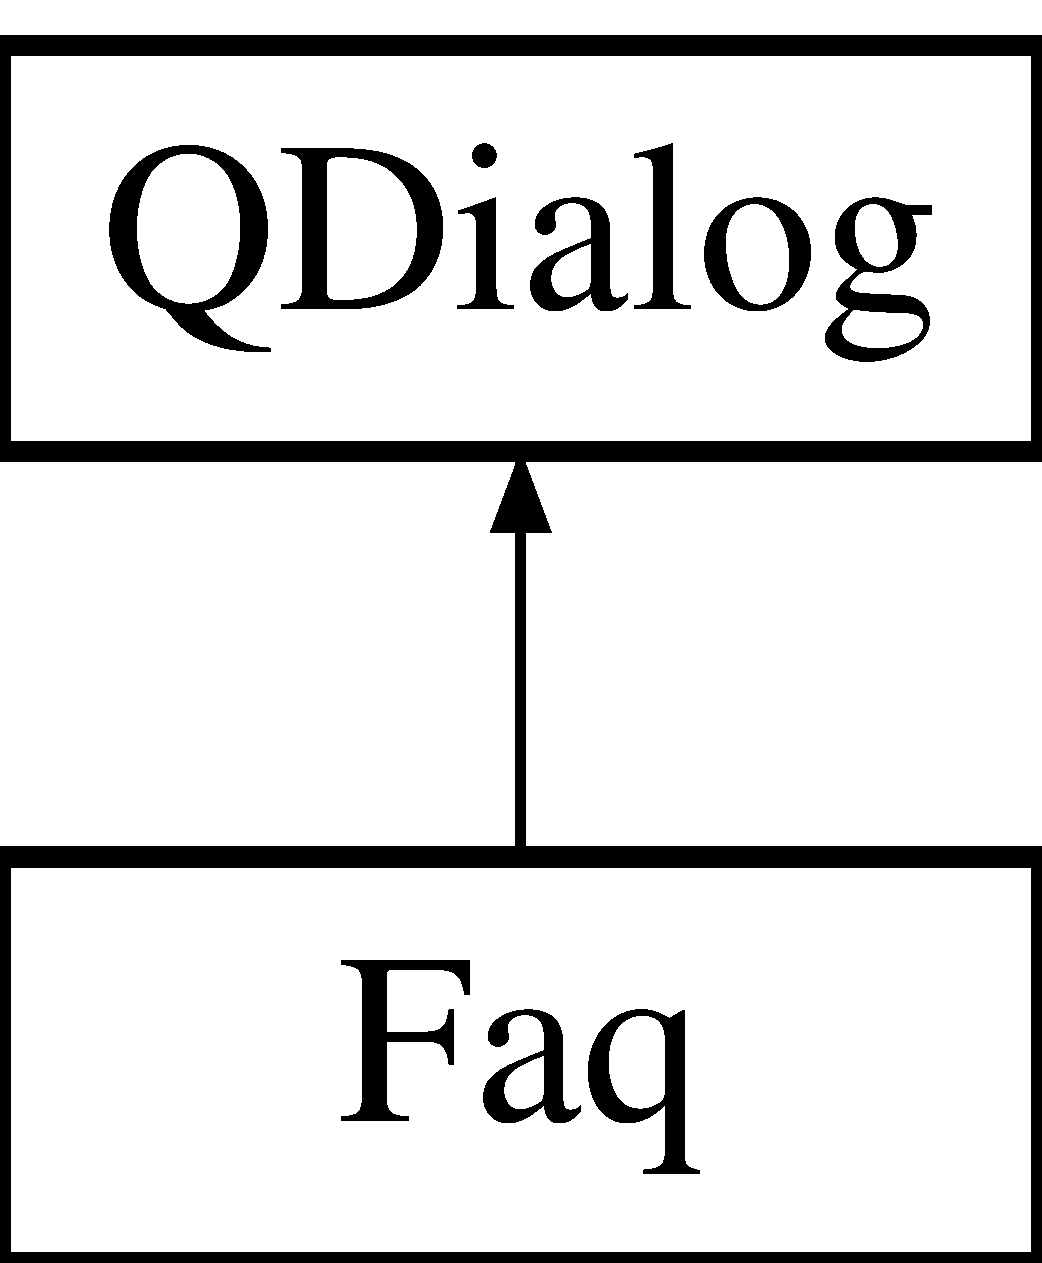
\includegraphics[height=2.000000cm]{class_faq}
\end{center}
\end{figure}
\subsection*{Fonctions membres publiques}
\begin{DoxyCompactItemize}
\item 
{\bf Faq} (Q\-Widget $\ast$parent)
\begin{DoxyCompactList}\small\item\em Cette classe permet d'ouvrir une fenetre \char`\"{}\-F\-A\-Q\char`\"{} en français ainsi quand anglais, qui permet a l'utilisateur de \subsubsection*{coomprendre l'utilisation de l'application }



 \end{DoxyCompactList}\end{DoxyCompactItemize}


\subsection{Documentation des constructeurs et destructeur}
\index{Faq@{Faq}!Faq@{Faq}}
\index{Faq@{Faq}!Faq@{Faq}}
\subsubsection[{Faq}]{\setlength{\rightskip}{0pt plus 5cm}Faq\-::\-Faq (
\begin{DoxyParamCaption}
\item[{Q\-Widget $\ast$}]{parent}
\end{DoxyParamCaption}
)}\label{class_faq_afda373b0c94a7f0c683dbef46888e3f0}


Cette classe permet d'ouvrir une fenetre \char`\"{}\-F\-A\-Q\char`\"{} en français ainsi quand anglais, qui permet a l'utilisateur de \subsubsection*{coomprendre l'utilisation de l'application }



 

\subsubsection*{Ize\-Nogoud }

\begin{DoxyDate}{Date}
24 Mars 2015 
\end{DoxyDate}
Ajoute le titre de la fenetre

Création d'un widget pour les onglets

fixe la position et la taille du widget

Création des labels ou le texte apparaitra

Insertion du texte en français

Insertion du texte en anglais

Ajoute les textes dans le widget des onglets 

La documentation de cette classe a été générée à partir des fichiers suivants \-:\begin{DoxyCompactItemize}
\item 
faq.\-h\item 
faq.\-cpp\end{DoxyCompactItemize}

\section{Référence de la classe Help}
\label{class_help}\index{Help@{Help}}
Graphe d'héritage de Help\-:\begin{figure}[H]
\begin{center}
\leavevmode
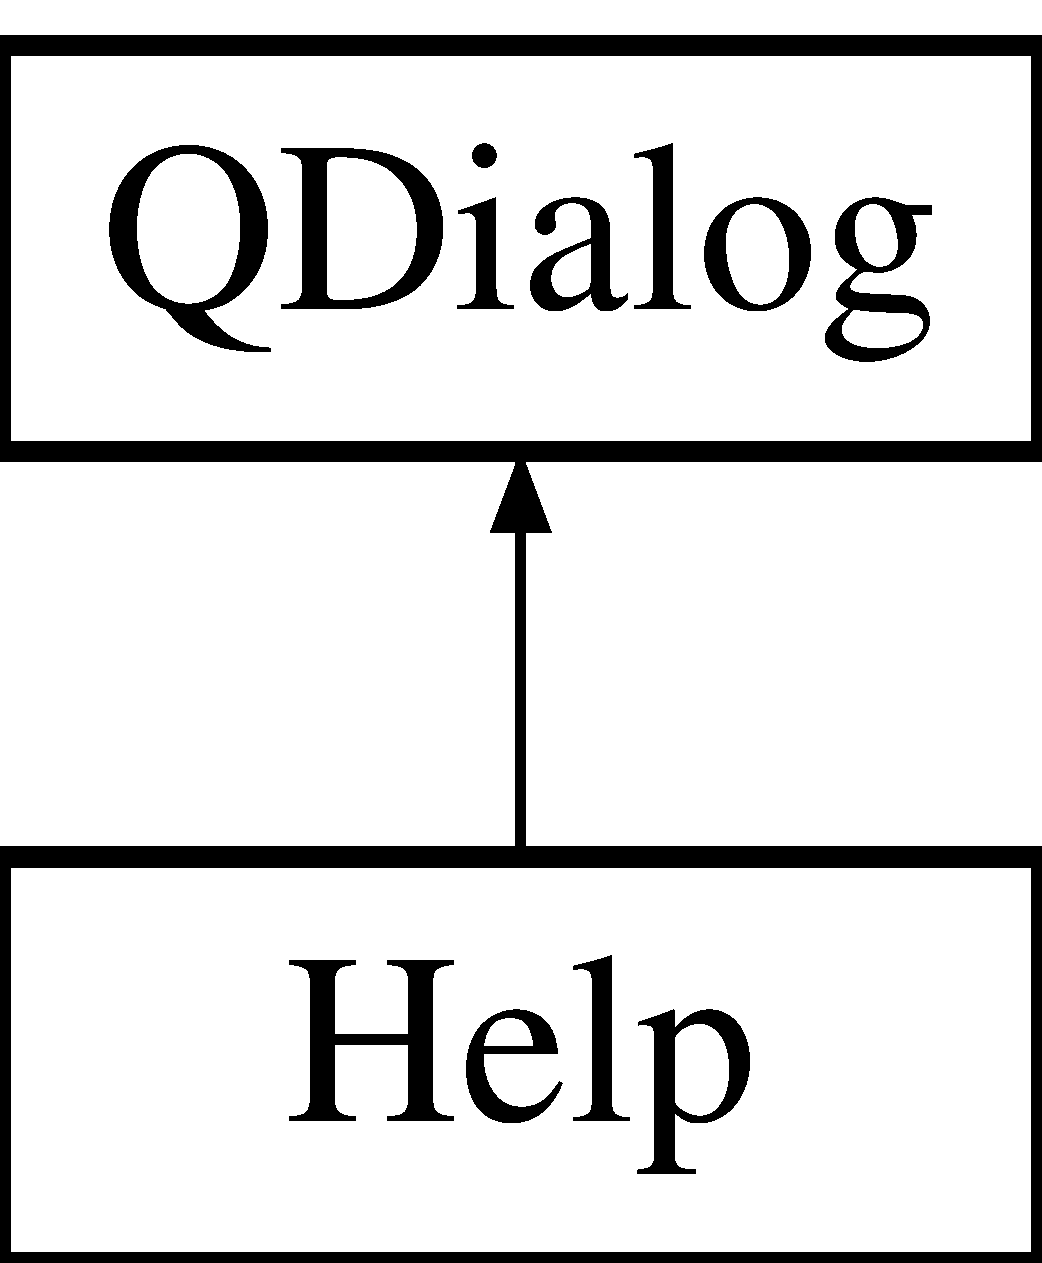
\includegraphics[height=2.000000cm]{class_help}
\end{center}
\end{figure}
\subsection*{Fonctions membres publiques}
\begin{DoxyCompactItemize}
\item 
{\bf Help} (Q\-Widget $\ast$parent)
\end{DoxyCompactItemize}


\subsection{Documentation des constructeurs et destructeur}
\index{Help@{Help}!Help@{Help}}
\index{Help@{Help}!Help@{Help}}
\subsubsection[{Help}]{\setlength{\rightskip}{0pt plus 5cm}Help\-::\-Help (
\begin{DoxyParamCaption}
\item[{Q\-Widget $\ast$}]{parent = {\ttfamily 0}}
\end{DoxyParamCaption}
)}\label{class_help_a9ce7c06caf8de0eb2aaae811fdd723fc}
Titre de la fenetre

Création d'un widget pour les onglets

fixe la position et la taille du widget

Création des labels ou le texte apparaitra

Insertion du texte en français

Insertion du texte en anglais

Ajoute les textes dans le widget des onglets 

La documentation de cette classe a été générée à partir des fichiers suivants \-:\begin{DoxyCompactItemize}
\item 
help.\-h\item 
help.\-cpp\end{DoxyCompactItemize}

\hypertarget{class_main_window}{\section{Référence de la classe Main\-Window}
\label{class_main_window}\index{Main\-Window@{Main\-Window}}
}


{\ttfamily \#include $<$mainwindow.\-h$>$}

Graphe d'héritage de Main\-Window\-:\begin{figure}[H]
\begin{center}
\leavevmode
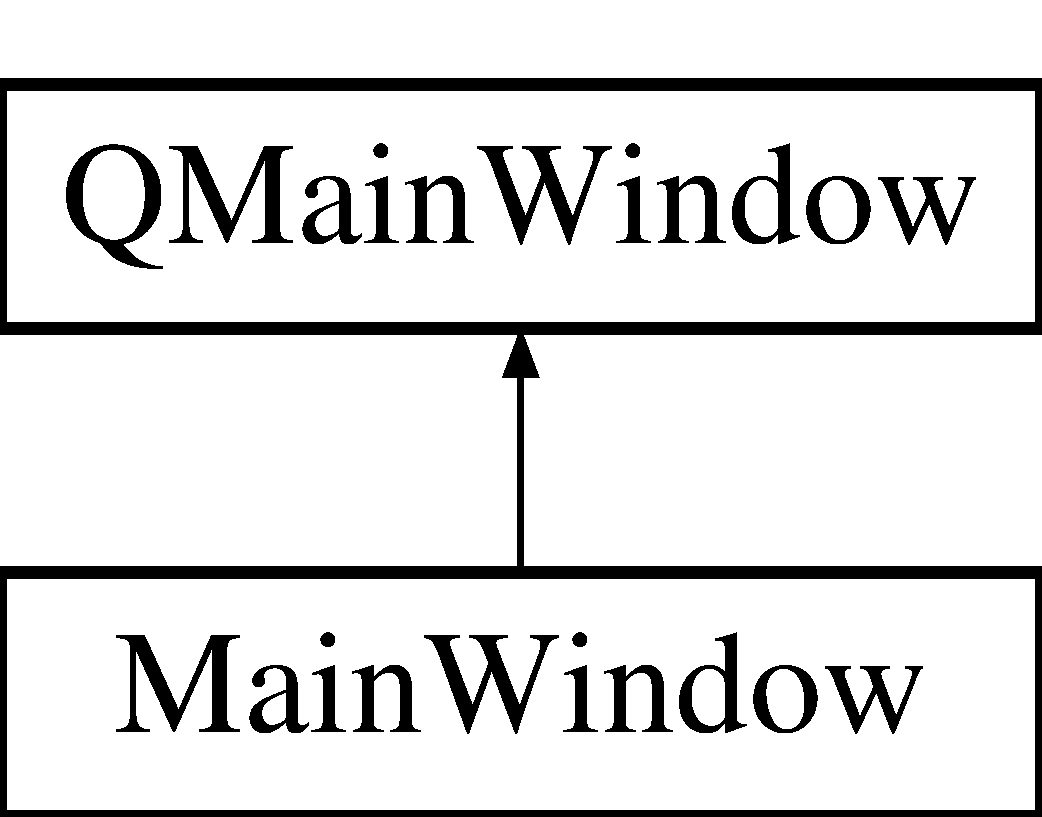
\includegraphics[height=2.000000cm]{class_main_window}
\end{center}
\end{figure}
\subsection*{Connecteurs publics}
\begin{DoxyCompactItemize}
\item 
void \hyperlink{class_main_window_acb789dac6a35383ad1d7bb6f652c7cee}{About} ()
\item 
void \hyperlink{class_main_window_a60313e11853d62369dd7f48c36867733}{Aide} ()
\item 
void \hyperlink{class_main_window_af71514a6d74571f32a45fa79ddd7d291}{show\-Eur\-Usd} ()
\item 
void \hyperlink{class_main_window_a3350e0511efc29d592d876a7298123c7}{show\-Eur\-Chf} ()
\item 
void \hyperlink{class_main_window_a80a42469b3b6fc9548123fdcb9c400db}{config\-Url} ()
\item 
void \hyperlink{class_main_window_adddc34c97edbe78434e600cdb076ebc7}{element\-Search} ()
\item 
void \hyperlink{class_main_window_a479a75cb750744fa76646781b6a96f79}{load\-Web\-View} ()
\end{DoxyCompactItemize}
\subsection*{Fonctions membres publiques}
\begin{DoxyCompactItemize}
\item 
\hyperlink{class_main_window_a8b244be8b7b7db1b08de2a2acb9409db}{Main\-Window} (Q\-Widget $\ast$parent=0)
\item 
\hyperlink{class_main_window_ae98d00a93bc118200eeef9f9bba1dba7}{$\sim$\-Main\-Window} ()
\end{DoxyCompactItemize}


\subsection{Documentation des constructeurs et destructeur}
\hypertarget{class_main_window_a8b244be8b7b7db1b08de2a2acb9409db}{\index{Main\-Window@{Main\-Window}!Main\-Window@{Main\-Window}}
\index{Main\-Window@{Main\-Window}!MainWindow@{Main\-Window}}
\subsubsection[{Main\-Window}]{\setlength{\rightskip}{0pt plus 5cm}Main\-Window\-::\-Main\-Window (
\begin{DoxyParamCaption}
\item[{Q\-Widget $\ast$}]{parent = {\ttfamily 0}}
\end{DoxyParamCaption}
)}}\label{class_main_window_a8b244be8b7b7db1b08de2a2acb9409db}
Fixe des dimensions à l'ouverture de la fenêtre principale, et indique le titre de la fenêtre.

Ajout d'une image à l'ouverture de l'application

Ajoute une barre de menu et l'implémente

Ajoute des actions possible dans les options de la barre de menu

Le menu A propos

Le menu F\-A\-Q

Créer la connection lors du clic, pour afficher le tableau des cotations pour les devise Euros / Franc suisse

A la modification de la date de filtre, un signal est envoyé pour rafraichir et ré-\/afficher le tableau filtrer

Créer la connection lors du clic, pour afficher le tableau des cotations pour les devise Euros / Dollar

A la modification de la date de filtre, un signal est envoyé pour rafraichir et ré-\/afficher le tableau filtrer

Appel de la fonction load\-Web\-View qui charge une page web, et récupère les données désirées

Timer permettant de réactualiser les données télécharger toutes les 10 secondes \hypertarget{class_main_window_ae98d00a93bc118200eeef9f9bba1dba7}{\index{Main\-Window@{Main\-Window}!$\sim$\-Main\-Window@{$\sim$\-Main\-Window}}
\index{$\sim$\-Main\-Window@{$\sim$\-Main\-Window}!MainWindow@{Main\-Window}}
\subsubsection[{$\sim$\-Main\-Window}]{\setlength{\rightskip}{0pt plus 5cm}Main\-Window\-::$\sim$\-Main\-Window (
\begin{DoxyParamCaption}
{}
\end{DoxyParamCaption}
)}}\label{class_main_window_ae98d00a93bc118200eeef9f9bba1dba7}


\subsection{Documentation des fonctions membres}
\hypertarget{class_main_window_acb789dac6a35383ad1d7bb6f652c7cee}{\index{Main\-Window@{Main\-Window}!About@{About}}
\index{About@{About}!MainWindow@{Main\-Window}}
\subsubsection[{About}]{\setlength{\rightskip}{0pt plus 5cm}void Main\-Window\-::\-About (
\begin{DoxyParamCaption}
{}
\end{DoxyParamCaption}
)\hspace{0.3cm}{\ttfamily [slot]}}}\label{class_main_window_acb789dac6a35383ad1d7bb6f652c7cee}
Appel la page A propos de \hypertarget{class_main_window_a60313e11853d62369dd7f48c36867733}{\index{Main\-Window@{Main\-Window}!Aide@{Aide}}
\index{Aide@{Aide}!MainWindow@{Main\-Window}}
\subsubsection[{Aide}]{\setlength{\rightskip}{0pt plus 5cm}void Main\-Window\-::\-Aide (
\begin{DoxyParamCaption}
{}
\end{DoxyParamCaption}
)\hspace{0.3cm}{\ttfamily [slot]}}}\label{class_main_window_a60313e11853d62369dd7f48c36867733}
Appel la page F\-A\-Q \hypertarget{class_main_window_a80a42469b3b6fc9548123fdcb9c400db}{\index{Main\-Window@{Main\-Window}!config\-Url@{config\-Url}}
\index{config\-Url@{config\-Url}!MainWindow@{Main\-Window}}
\subsubsection[{config\-Url}]{\setlength{\rightskip}{0pt plus 5cm}void Main\-Window\-::config\-Url (
\begin{DoxyParamCaption}
{}
\end{DoxyParamCaption}
)\hspace{0.3cm}{\ttfamily [slot]}}}\label{class_main_window_a80a42469b3b6fc9548123fdcb9c400db}
Appel la page configuration \hypertarget{class_main_window_adddc34c97edbe78434e600cdb076ebc7}{\index{Main\-Window@{Main\-Window}!element\-Search@{element\-Search}}
\index{element\-Search@{element\-Search}!MainWindow@{Main\-Window}}
\subsubsection[{element\-Search}]{\setlength{\rightskip}{0pt plus 5cm}void Main\-Window\-::element\-Search (
\begin{DoxyParamCaption}
{}
\end{DoxyParamCaption}
)\hspace{0.3cm}{\ttfamily [slot]}}}\label{class_main_window_adddc34c97edbe78434e600cdb076ebc7}
Recherche dans la page les lignes du tableau uis chaque colone afin de la rentré dans la base de données connection a la base pour l'insertion

récupère le corp de la page pour pouvoir le manipuler

Récupère toute les lignes (tr)

Boucle sur les lignes

Récupère toutes les colonnes (td)

Ajoute les données récupérer dans les bon champs de la base de données

Vérifie les dernière données de la base pour éviter les doublons \hypertarget{class_main_window_a479a75cb750744fa76646781b6a96f79}{\index{Main\-Window@{Main\-Window}!load\-Web\-View@{load\-Web\-View}}
\index{load\-Web\-View@{load\-Web\-View}!MainWindow@{Main\-Window}}
\subsubsection[{load\-Web\-View}]{\setlength{\rightskip}{0pt plus 5cm}void Main\-Window\-::load\-Web\-View (
\begin{DoxyParamCaption}
{}
\end{DoxyParamCaption}
)\hspace{0.3cm}{\ttfamily [slot]}}}\label{class_main_window_a479a75cb750744fa76646781b6a96f79}
Charge la page entière de l'U\-R\-L renseignée Concatène l'identification des cotations cocher à l'url pour le téléchargement des données

Crée un webview et charge l'url renseigné + les cotations cocher

Appel un slot à la fin du chargement

cache le widget généré \hypertarget{class_main_window_a3350e0511efc29d592d876a7298123c7}{\index{Main\-Window@{Main\-Window}!show\-Eur\-Chf@{show\-Eur\-Chf}}
\index{show\-Eur\-Chf@{show\-Eur\-Chf}!MainWindow@{Main\-Window}}
\subsubsection[{show\-Eur\-Chf}]{\setlength{\rightskip}{0pt plus 5cm}void Main\-Window\-::show\-Eur\-Chf (
\begin{DoxyParamCaption}
{}
\end{DoxyParamCaption}
)\hspace{0.3cm}{\ttfamily [slot]}}}\label{class_main_window_a3350e0511efc29d592d876a7298123c7}
Affiche le tableau de devise euro / franc suisse \hypertarget{class_main_window_af71514a6d74571f32a45fa79ddd7d291}{\index{Main\-Window@{Main\-Window}!show\-Eur\-Usd@{show\-Eur\-Usd}}
\index{show\-Eur\-Usd@{show\-Eur\-Usd}!MainWindow@{Main\-Window}}
\subsubsection[{show\-Eur\-Usd}]{\setlength{\rightskip}{0pt plus 5cm}void Main\-Window\-::show\-Eur\-Usd (
\begin{DoxyParamCaption}
{}
\end{DoxyParamCaption}
)\hspace{0.3cm}{\ttfamily [slot]}}}\label{class_main_window_af71514a6d74571f32a45fa79ddd7d291}
Affiche le tableau de devise euro / dollar 

La documentation de cette classe a été générée à partir des fichiers suivants \-:\begin{DoxyCompactItemize}
\item 
\hyperlink{mainwindow_8h}{mainwindow.\-h}\item 
\hyperlink{mainwindow_8cpp}{mainwindow.\-cpp}\end{DoxyCompactItemize}

\chapter{Documentation des fichiers}
\hypertarget{aide_8cpp}{\section{Référence du fichier aide.\-cpp}
\label{aide_8cpp}\index{aide.\-cpp@{aide.\-cpp}}
}
{\ttfamily \#include \char`\"{}aide.\-h\char`\"{}}\\*

\hypertarget{aide_8h}{\section{Référence du fichier aide.\-h}
\label{aide_8h}\index{aide.\-h@{aide.\-h}}
}
\subsection*{Classes}
\begin{DoxyCompactItemize}
\item 
class \hyperlink{class_aide}{Aide}
\end{DoxyCompactItemize}

\hypertarget{config_8cpp}{\section{Référence du fichier config.\-cpp}
\label{config_8cpp}\index{config.\-cpp@{config.\-cpp}}
}
{\ttfamily \#include \char`\"{}config.\-h\char`\"{}}\\*
{\ttfamily \#include \char`\"{}mainwindow.\-h\char`\"{}}\\*
{\ttfamily \#include $<$Q\-Check\-Box$>$}\\*
{\ttfamily \#include $<$Q\-Dialog$>$}\\*
{\ttfamily \#include $<$Q\-Form\-Layout$>$}\\*
{\ttfamily \#include $<$Q\-Group\-Box$>$}\\*
{\ttfamily \#include $<$Q\-Line\-Edit$>$}\\*
{\ttfamily \#include $<$Q\-V\-Box\-Layout$>$}\\*
{\ttfamily \#include $<$Q\-Dir$>$}\\*

\hypertarget{config_8h}{\section{Référence du fichier config.\-h}
\label{config_8h}\index{config.\-h@{config.\-h}}
}
{\ttfamily \#include $<$Q\-Dialog$>$}\\*
{\ttfamily \#include $<$Q\-Settings$>$}\\*
\subsection*{Classes}
\begin{DoxyCompactItemize}
\item 
class \hyperlink{class_config}{Config}
\end{DoxyCompactItemize}

\hypertarget{connectiondb_8cpp}{\section{Référence du fichier connectiondb.\-cpp}
\label{connectiondb_8cpp}\index{connectiondb.\-cpp@{connectiondb.\-cpp}}
}
{\ttfamily \#include \char`\"{}connectiondb.\-h\char`\"{}}\\*
{\ttfamily \#include \char`\"{}mainwindow.\-h\char`\"{}}\\*
{\ttfamily \#include $<$Q\-Sql\-Database$>$}\\*
{\ttfamily \#include $<$Q\-Message\-Box$>$}\\*
{\ttfamily \#include $<$Q\-Debug$>$}\\*
{\ttfamily \#include $<$Q\-Sql\-Table\-Model$>$}\\*
{\ttfamily \#include $<$Q\-Sql\-Error$>$}\\*
{\ttfamily \#include $<$Qt\-Sql/\-Q\-Sql\-Database$>$}\\*
{\ttfamily \#include $<$Q\-Table\-View$>$}\\*
{\ttfamily \#include $<$Q\-Sql\-Query$>$}\\*
{\ttfamily \#include $<$Q\-Network\-Request$>$}\\*
{\ttfamily \#include $<$Q\-Web\-Frame$>$}\\*

\hypertarget{connectiondb_8h}{\section{Référence du fichier connectiondb.\-h}
\label{connectiondb_8h}\index{connectiondb.\-h@{connectiondb.\-h}}
}
{\ttfamily \#include $<$Q\-Sql\-Database$>$}\\*
{\ttfamily \#include $<$Q\-V\-Box\-Layout$>$}\\*
{\ttfamily \#include $<$Q\-Network\-Access\-Manager$>$}\\*
{\ttfamily \#include $<$Q\-Web\-Page$>$}\\*
{\ttfamily \#include $<$Q\-Web\-View$>$}\\*
{\ttfamily \#include $<$Q\-Web\-Element$>$}\\*
\subsection*{Classes}
\begin{DoxyCompactItemize}
\item 
class \hyperlink{class_connection_d_b}{Connection\-D\-B}
\end{DoxyCompactItemize}

\hypertarget{faq_8cpp}{\section{Référence du fichier faq.\-cpp}
\label{faq_8cpp}\index{faq.\-cpp@{faq.\-cpp}}
}
{\ttfamily \#include \char`\"{}faq.\-h\char`\"{}}\\*
{\ttfamily \#include $<$Q\-Label$>$}\\*
{\ttfamily \#include $<$Q\-V\-Box\-Layout$>$}\\*
{\ttfamily \#include $<$Qt\-Widgets$>$}\\*

\hypertarget{faq_8h}{\section{Référence du fichier faq.\-h}
\label{faq_8h}\index{faq.\-h@{faq.\-h}}
}
{\ttfamily \#include $<$Q\-Dialog$>$}\\*
\subsection*{Classes}
\begin{DoxyCompactItemize}
\item 
class \hyperlink{class_faq}{Faq}
\end{DoxyCompactItemize}

\hypertarget{help_8cpp}{\section{Référence du fichier help.\-cpp}
\label{help_8cpp}\index{help.\-cpp@{help.\-cpp}}
}
{\ttfamily \#include \char`\"{}help.\-h\char`\"{}}\\*
{\ttfamily \#include $<$Q\-Label$>$}\\*
{\ttfamily \#include $<$Q\-Tab\-Widget$>$}\\*
{\ttfamily \#include $<$Q\-V\-Box\-Layout$>$}\\*

\hypertarget{help_8h}{\section{Référence du fichier help.\-h}
\label{help_8h}\index{help.\-h@{help.\-h}}
}
{\ttfamily \#include $<$Q\-Dialog$>$}\\*
\subsection*{Classes}
\begin{DoxyCompactItemize}
\item 
class \hyperlink{class_help}{Help}
\end{DoxyCompactItemize}

\hypertarget{main_8cpp}{\section{Référence du fichier main.\-cpp}
\label{main_8cpp}\index{main.\-cpp@{main.\-cpp}}
}
{\ttfamily \#include $<$Q\-Application$>$}\\*
{\ttfamily \#include \char`\"{}mainwindow.\-h\char`\"{}}\\*
\subsection*{Macros}
\begin{DoxyCompactItemize}
\item 
\#define \hyperlink{main_8cpp_ad4dd36de8176cf839bc095ffcc419ebb}{q2c}(string)~string.\-to\-Std\-String()
\end{DoxyCompactItemize}
\subsection*{Fonctions}
\begin{DoxyCompactItemize}
\item 
int \hyperlink{main_8cpp_a0ddf1224851353fc92bfbff6f499fa97}{main} (int argc, char $\ast$argv\mbox{[}$\,$\mbox{]})
\end{DoxyCompactItemize}


\subsection{Documentation des macros}
\hypertarget{main_8cpp_ad4dd36de8176cf839bc095ffcc419ebb}{\index{main.\-cpp@{main.\-cpp}!q2c@{q2c}}
\index{q2c@{q2c}!main.cpp@{main.\-cpp}}
\subsubsection[{q2c}]{\setlength{\rightskip}{0pt plus 5cm}\#define q2c(
\begin{DoxyParamCaption}
\item[{}]{string}
\end{DoxyParamCaption}
)~string.\-to\-Std\-String()}}\label{main_8cpp_ad4dd36de8176cf839bc095ffcc419ebb}


\subsection{Documentation des fonctions}
\hypertarget{main_8cpp_a0ddf1224851353fc92bfbff6f499fa97}{\index{main.\-cpp@{main.\-cpp}!main@{main}}
\index{main@{main}!main.cpp@{main.\-cpp}}
\subsubsection[{main}]{\setlength{\rightskip}{0pt plus 5cm}int main (
\begin{DoxyParamCaption}
\item[{int}]{argc, }
\item[{char $\ast$}]{argv\mbox{[}$\,$\mbox{]}}
\end{DoxyParamCaption}
)}}\label{main_8cpp_a0ddf1224851353fc92bfbff6f499fa97}

\hypertarget{mainwindow_8cpp}{\section{Référence du fichier mainwindow.\-cpp}
\label{mainwindow_8cpp}\index{mainwindow.\-cpp@{mainwindow.\-cpp}}
}
{\ttfamily \#include \char`\"{}mainwindow.\-h\char`\"{}}\\*
{\ttfamily \#include \char`\"{}connectiondb.\-h\char`\"{}}\\*
{\ttfamily \#include \char`\"{}help.\-h\char`\"{}}\\*
{\ttfamily \#include \char`\"{}faq.\-h\char`\"{}}\\*
{\ttfamily \#include \char`\"{}config.\-h\char`\"{}}\\*
{\ttfamily \#include $<$Q\-Web\-Element$>$}\\*
{\ttfamily \#include $<$Q\-Web\-Frame$>$}\\*
{\ttfamily \#include $<$Q\-Network\-Access\-Manager$>$}\\*
{\ttfamily \#include $<$Q\-Sql\-Query$>$}\\*
{\ttfamily \#include $<$Q\-Sql\-Record$>$}\\*
{\ttfamily \#include $<$Q\-I\-O\-Device$>$}\\*
{\ttfamily \#include $<$Q\-Settings$>$}\\*
{\ttfamily \#include $<$Q\-Xml\-Stream\-Reader$>$}\\*
{\ttfamily \#include $<$Q\-String$>$}\\*
{\ttfamily \#include $<$Q\-Sql\-Query\-Model$>$}\\*
\subsection*{Fonctions}
\begin{DoxyCompactItemize}
\item 
bool \hyperlink{mainwindow_8cpp_a3d9bc2a0506ed995cc633411e240ac2d}{read\-Xml\-File} (Q\-I\-O\-Device \&device, Q\-Settings\-::\-Settings\-Map \&map)
\item 
bool \hyperlink{mainwindow_8cpp_acc040234bba2e5f0ef9a97ea45d9f254}{write\-Xml\-File} (Q\-I\-O\-Device \&device, const Q\-Settings\-::\-Settings\-Map \&map)
\end{DoxyCompactItemize}


\subsection{Documentation des fonctions}
\hypertarget{mainwindow_8cpp_a3d9bc2a0506ed995cc633411e240ac2d}{\index{mainwindow.\-cpp@{mainwindow.\-cpp}!read\-Xml\-File@{read\-Xml\-File}}
\index{read\-Xml\-File@{read\-Xml\-File}!mainwindow.cpp@{mainwindow.\-cpp}}
\subsubsection[{read\-Xml\-File}]{\setlength{\rightskip}{0pt plus 5cm}bool read\-Xml\-File (
\begin{DoxyParamCaption}
\item[{Q\-I\-O\-Device \&}]{device, }
\item[{Q\-Settings\-::\-Settings\-Map \&}]{map}
\end{DoxyParamCaption}
)}}\label{mainwindow_8cpp_a3d9bc2a0506ed995cc633411e240ac2d}
Fonction permettant de lire un fichier Xml \hypertarget{mainwindow_8cpp_acc040234bba2e5f0ef9a97ea45d9f254}{\index{mainwindow.\-cpp@{mainwindow.\-cpp}!write\-Xml\-File@{write\-Xml\-File}}
\index{write\-Xml\-File@{write\-Xml\-File}!mainwindow.cpp@{mainwindow.\-cpp}}
\subsubsection[{write\-Xml\-File}]{\setlength{\rightskip}{0pt plus 5cm}bool write\-Xml\-File (
\begin{DoxyParamCaption}
\item[{Q\-I\-O\-Device \&}]{device, }
\item[{const Q\-Settings\-::\-Settings\-Map \&}]{map}
\end{DoxyParamCaption}
)}}\label{mainwindow_8cpp_acc040234bba2e5f0ef9a97ea45d9f254}
Fonction permettant d'écrire dans un fichier Xml 
\hypertarget{mainwindow_8h}{\section{Référence du fichier mainwindow.\-h}
\label{mainwindow_8h}\index{mainwindow.\-h@{mainwindow.\-h}}
}
{\ttfamily \#include $<$Q\-Main\-Window$>$}\\*
{\ttfamily \#include $<$Qt\-Widgets$>$}\\*
{\ttfamily \#include $<$Q\-Push\-Button$>$}\\*
{\ttfamily \#include $<$Q\-Web\-Element$>$}\\*
{\ttfamily \#include $<$Q\-Sql\-Database$>$}\\*
{\ttfamily \#include $<$Qt\-Web\-Kit\-Widgets/\-Q\-Web\-View$>$}\\*
\subsection*{Classes}
\begin{DoxyCompactItemize}
\item 
class \hyperlink{class_main_window}{Main\-Window}
\end{DoxyCompactItemize}
\subsection*{Fonctions}
\begin{DoxyCompactItemize}
\item 
bool \hyperlink{mainwindow_8h_a3d9bc2a0506ed995cc633411e240ac2d}{read\-Xml\-File} (Q\-I\-O\-Device \&device, Q\-Settings\-::\-Settings\-Map \&map)
\item 
bool \hyperlink{mainwindow_8h_acc040234bba2e5f0ef9a97ea45d9f254}{write\-Xml\-File} (Q\-I\-O\-Device \&device, const Q\-Settings\-::\-Settings\-Map \&map)
\end{DoxyCompactItemize}


\subsection{Documentation des fonctions}
\hypertarget{mainwindow_8h_a3d9bc2a0506ed995cc633411e240ac2d}{\index{mainwindow.\-h@{mainwindow.\-h}!read\-Xml\-File@{read\-Xml\-File}}
\index{read\-Xml\-File@{read\-Xml\-File}!mainwindow.h@{mainwindow.\-h}}
\subsubsection[{read\-Xml\-File}]{\setlength{\rightskip}{0pt plus 5cm}bool read\-Xml\-File (
\begin{DoxyParamCaption}
\item[{Q\-I\-O\-Device \&}]{device, }
\item[{Q\-Settings\-::\-Settings\-Map \&}]{map}
\end{DoxyParamCaption}
)}}\label{mainwindow_8h_a3d9bc2a0506ed995cc633411e240ac2d}
Fonction pour la lecture et l'ecriture des données dans un fichier Xml

Fonction permettant de lire un fichier Xml \hypertarget{mainwindow_8h_acc040234bba2e5f0ef9a97ea45d9f254}{\index{mainwindow.\-h@{mainwindow.\-h}!write\-Xml\-File@{write\-Xml\-File}}
\index{write\-Xml\-File@{write\-Xml\-File}!mainwindow.h@{mainwindow.\-h}}
\subsubsection[{write\-Xml\-File}]{\setlength{\rightskip}{0pt plus 5cm}bool write\-Xml\-File (
\begin{DoxyParamCaption}
\item[{Q\-I\-O\-Device \&}]{device, }
\item[{const Q\-Settings\-::\-Settings\-Map \&}]{map}
\end{DoxyParamCaption}
)}}\label{mainwindow_8h_acc040234bba2e5f0ef9a97ea45d9f254}
Fonction permettant d'écrire dans un fichier Xml 
%--- End generated contents ---

% Index
\newpage
\phantomsection
\addcontentsline{toc}{chapter}{Index}
\printindex

\end{document}
